\documentclass[10pt,a4paper]{article}
\usepackage[utf8]{inputenc}
\usepackage[italian]{babel}
\usepackage{amsmath}
\usepackage{xcolor}
\usepackage{circuitikz}
\usepackage{amsfonts}
\usepackage{amssymb}
\usepackage{graphicx}
\usepackage[left=2cm,right=2cm,top=2cm,bottom=2cm]{geometry}
\newcommand{\rem}[1]{[\emph{#1}]}
\newcommand{\exn}{\phantom{xxx}}
\renewcommand{\thesubsection}{\thesection.\alph{subsection}}  %% use 1.a numbering

\author{Gruppo 1G.BN \\ Massimo Bilancioni, Alessandro Foligno, Giuseppe Zanichelli }
\title{Es05B: Circuiti lineari con Amplificatori Operazionali}
\begin{document}
	\date{8 novembre 2018}
	\maketitle
	
	
	\section*{Scopo dell' esperienza}
	Misurare le caratteristiche di circuiti lineari realizzati con un op-amp TL081 alimentati tra +15 V e -15 V.
	
	\section{Amplificatore invertente}
	Si vuole realizzare un amplificatore invertente con un'~impedenza di ingresso superiore a 1 
	k$\Omega$ e con un amplificazione a centro banda di 10.
	
	\subsection{Scelta dei componenti}
	
	Si monta il circuito secondo lo schema mostrato in figura, utilizzando la barra di 
	distribuzione verde per la tensione negativa, quella rosso per la tensione positiva, e quella nera per 
	la massa.
	


	
	Le resistenze selezionate hanno i seguenti valori, misurati con il multimetro digitale, con il corrispondente valore atteso 
	del guadagno in tensione dell'~amplificatore.
	\[
	R_1 = ( 1.466 \pm 0.012) \,\mathrm{k}\Omega, \quad 
	R_2 = (15.24  \pm 0.12) \,\mathrm{k}\Omega, \quad 
	A_{exp} = -(10.39 \pm 0.11)
	\]
	
	\subsection{Montaggio circuito}
	Il circuito è stato montato nella basetta come riportato in figura.
	\begin{center}
		\begin{circuitikz}\draw
			(3,-0.5) node[op amp] (opamp) {}
			(opamp.-) to[R=R1] (0,-0)
			(2,0) --	(2,2) to[R=R2] (4.15,2) to(opamp.out) -- (6,-0.5) node[right] {$v_{out}$}
			(0,0) node[left] {\textnormal{$v_{in}$}}
			(opamp.up) --++(0,1) node[circ]{15\,\textnormal{V}}
			(opamp.down) --++(0,-2) node[circ] {} node[left]{  -15\,\textnormal{V}}
			
			(opamp.+) to (0,-1) node[ground] {};	
		\end{circuitikz}
	\end{center}
	
	%%%%%%%%%%%%%%%%%%%%%%%%%%%%%%%%%%%%%%%%%%%%%%%%%%%%%%
	\subsection{Linearit\`a e misura del guadagno}
	Si fissa la frequenza del segnale ad $f_{in} = (2.597 \pm 0.011)$ kHz e si invia all'~ingresso dell'~amplificatore.	L'uscita dell'~amplificatore \`e mostrata qualitativativamente in Fig. \ref{fig:oscinv} per due 
	differenti ampiezze di $V_{in}$ (circa $1.26$~Vpp e $7.20$~Vpp). 
	Nel primo caso l'~OpAmp si comporta in modo lineare mentre nel secondo caso si osserva clipping. Il datasheet riporta uno Slew rate di $13 V/\mu s$ che è quindi trascurabile a questa frequenza .
	%
	\begin{figure}[h]
		\begin{center}
		
			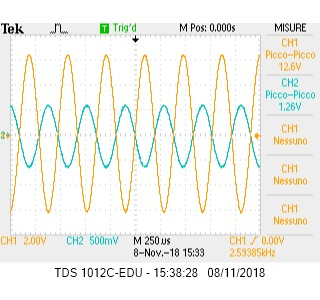
\includegraphics[scale=0.7]{foto1.jpg}
			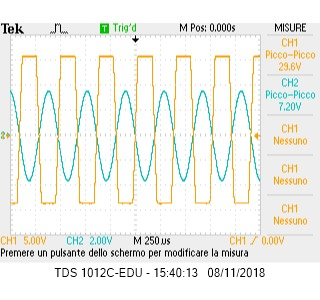
\includegraphics[scale=0.7]{foto2.jpg}
			\caption{screenshot dei segnali con e senza clipping}
			%\includegraphics[0.45\textwidth]{}
		\end{center}
		\caption{\small Ingresso (in alto) ed uscita (in basso) di un amplificatore invertente con OpAmp, in 
			zona lineare (a sinistra) e non (a destra)}
		\label{fig:oscinv}
	\end{figure}
	%
	
	Variando l'~ampiezza di $V_{in}$ si misura $V_{out}$ ed il relativo guadagno $A_V=V_{out}/V_{in}$ riportando i dati ottenuti in tabella~\ref{tab:guadagno} 
	e mostrandone un grafico in Fig. \ref{fit}. 
	Il fit è stato ottenuto mediante media pesata dei valori del guadagno; si può osservare come, alzando l'ampiezza, il guadagno diminuisca impercettibilmente. Trovandosi il tutto dentro una barra d'errore, non è considerabile un effetto significativo.
	L'incertezza sul guadagno è stato ottenuta sommando in quadratura le incertezze su Vin e Vout, dato che queste, essendo state misurate su canali diversi, si assumono scorrelate (anche l'incertezza sul digit è scorrelata).
	
	\begin{table}[h]
		\caption{$V_{out}$ in funzione di $V_{in}$ e relativo rapporto.}
		\label{tab:guadagno}
		\begin{center}
			\begin{tabular}{|c|c|c|}
				\hline
				$V_{in}$ (V) & $V_{out}$ (V)  & $A_V$ \\
				\hline
				\hline
				$ 0.50\pm 0.01 $ & $5.12 \pm 0.1 $ & $10.3 \pm 0.4 $ \\
				\hline
				$0.71 \pm 0.02 $ & $7.4 \pm 0.2 $ & $10.4 \pm 0.4 $ \\
				\hline
				$0.90 \pm 0.03 $ & $9.4 \pm 0.3 $ & $10.4 \pm 0.4 $ \\
				\hline
				$1.2 \pm 0.03 $ & $12.4 \pm 0.3 $ & $10.3 \pm 0.4 $ \\
				\hline
				$1.46 \pm 0.04 $ & $15.1 \pm 0.4 $ & $10.3 \pm 0.4 $ \\
				\hline
				$1.58 \pm 0.05 $ & $16.3 \pm 0.5 $ & $10.3 \pm 0.4 $ \\
				\hline
				$1.82 \pm 0.06 $ & $18.5 \pm 0.6 $ & $10.2 \pm 0.4 $ \\
				\hline
				$1.98 \pm 0.06 $ & $20.2 \pm 0.6 $ & $10.2 \pm 0.4 $ \\
				\hline
				$2.18 \pm 0.06 $ & $22.2 \pm 0.6 $ & $10.2 \pm 0.4 $ \\
				\hline
				$2.46 \pm 0.07 $ & $24.8 \pm 0.7 $ & $10.1 \pm 0.4 $ \\
				\hline
				$2.68 \pm 0.08 $ & $27.2 \pm 0.8 $ & $10.1 \pm 0.4 $ \\
				\hline
		
			\end{tabular}
		\end{center}
	\end{table}

		Gli ultimi 4 dati,riportati in tabella \ref{tab:daticlipping} sono stati presi per verificare il clipping, e quindi non considerati per il fit
		\begin{table}[h]
	
			\begin{center}
				\begin{tabular}{|c|c|c|}
					\hline
					$V_{in}$ (V) & $V_{out}$ (V)   \\
		\hline
		$2.96 \pm 0.09 $ & $28.8 \pm 0.8 $ \\
		\hline
		$3.04 \pm 0.09 $ & $29.3 \pm 0.8  $ \\
		\hline
		$3.20 \pm 0.09 $ & $29.4 \pm 0.9  $ \\
		\hline
		$3.25 \pm 0.1 $ & $29.5 \pm 0.9 $ \\
		\hline
		\end{tabular}
	\end{center}
\label{tab:daticlipping}
\caption{dati del segnale tagliato (clipping)}
\end{table}

	\begin{figure}\centering
			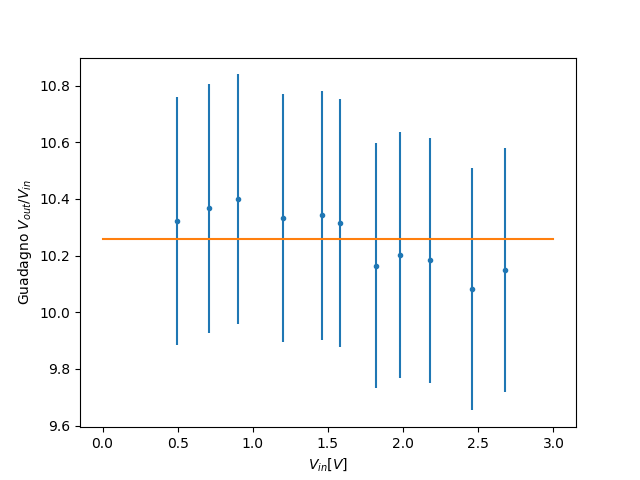
\includegraphics[scale=0.5]{fit.png}
				\caption{\small Linearit\`a dell'~amplificatore invertente}
			\label{fit}
	\end{figure}

	
	Si determina il guadagno mediante fit dei dati ottenuti:
	\[
	A_{best} = 10.258 \pm 0.001 \quad  \chi^2/ndof = 0.06
	\]

	Quindi gli errori sono stati sovrastimati.
	Cambiando la tensione dell'integrato si osserva clipping circa quando la tensione in uscita è pari a quella di alimentazione (in realtà un po' prima).
	
	%%%%%%%%%%%%%%%%%%
	%
	\section{Risposta in frequenza e \emph{slew rate}}
	\subsection{Risposta in frequenza del circuito}
	Non siamo riusciti a vedere la frequenza di taglio inferiore, che tuttavia deve essere   $ <10\mathrm{Hz}$ visto che per questa frequenza  non si ha una sensibile diminuzione del guadagno.

 Per la frequenza di taglio superiore abbiamo campionato il guadagno per frequenze tra $1\mathrm{kHz}$ e $ 1\mathrm{MHz}.$
Abbiamo abbassato $V_{in}$ per alte frequenze per evitare per evitare  possibili Slew Rate.

La frequenza di taglio è stata ricavata come l'intersezione delle due rette fittate rispettivamente a bassa e ad alta frequenza.
(Figura \ref{fig:bodeinv})

\textcolor{red}{errore su fH e dire pendenza per grandi omega}

	
	\[
	f_H = (167.7 \pm \exn \;)\,\mathrm{kHz}
	\]
	\begin{table}[h]
		\caption{\small Guadagno dell'~amplificatore invertente in funzione della frequenza.}
		\label{tab:bodeinv}
		\begin{center}
			\begin{tabular}{|c|c|c|c|}	\hline
				$f_{in}$ (kHz) & $V_{in}$ (V) & $V_{out}$ (V) & $A$ (dB) \\
				\hline
				$\exn0.753 \pm0.015 \exn $ & $\exn1.02 \pm 0.03\exn$ & $\exn10.4 \pm 0.3 \exn $ & $\exn 20.2\pm 0.26\exn $\\
				\hline
				$\exn 1.76\pm 0.04\exn $ & $\exn1.03\pm 0.03\exn$ & $\exn 10.5\pm 0.3\exn $ & $\exn 20.2\pm0.26 \exn $\\
\hline


			
				$\exn 2.90\pm0.06 \exn $ & $\exn1.03 \pm 0.03\exn$ & $\exn 10.5\pm 0.3 \exn $ & $\exn 20.2\pm0.26 \exn $\\
				\hline
				$\exn 6.22\pm0.12 \exn $ & $\exn1.05 \pm0.03 \exn $& $\exn 10.7\pm 0.3 \exn $ & $\exn 20.2\pm0.26 \exn $\\
				\hline
				$\exn 12.2\pm 0.2\exn $  & $\exn1.06 \pm0.03 \exn$& $\exn 10.7\pm 0.3 \exn $ & $\exn 20.1\pm0.26 \exn $\\
				\hline
				$\exn22.5 \pm 0.4\exn $ & $\exn1.05\pm0.03 \exn $& $\exn 10.6\pm 0.3 \exn $ & $\exn20.1\pm0.26 \exn $\\
				\hline
				$\exn44.9 \pm0.9 \exn $ & $\exn1.05 \pm 0.03\exn$ & $\exn10.5 \pm 0.3 \exn $ & $\exn 20.0\pm0.26 \exn $\\
				\hline
				$\exn 86.7\pm1.7 \exn $ & $\exn1.06 \pm 0.03\exn$ & $\exn9.92 \pm 0.3 \exn $ & $\exn 19.4\pm0.26 \exn $\\
				\hline
				$\exn 166\pm 3\exn $  & $\exn1.06 \pm 0.03\exn$& $\exn8.48 \pm 0.3 \exn $ & $\exn 18.1 \pm0.26 \exn $\\
  \hline
				$\exn212\pm  4\exn $ & $\exn 0.688\pm 0.02 \exn$ & $\exn4.96 \pm 0.15\exn $ & $\exn 17.2\pm 0.26 \exn $\\

\hline
				$\exn251 \pm 5 \exn $  & $\exn0.680 \pm 0.02\exn$& $\exn4.44 \pm0.14 \exn $ & $\exn 16.3\pm 0.26 \exn $\\
				\hline
				$\exn 350\pm 7\exn $  & $\exn0.776 \pm 0.02\exn$& $\exn 4.02\pm 0.13\exn $ & $\exn14.3\pm0.26 \exn $\\
				\hline
				$\exn 435\pm 9 \exn $ & $\exn0.688\pm0.02 \exn$ & $\exn 3.00\pm 0.09 \exn $ & $\exn 12.8\pm0.26 \exn $\\
				\hline
				$\exn555 \pm 10  \exn $ & $\exn0.696 \pm0.02 \exn$ & $\exn2.44 \pm 0.08\exn $ & $\exn 10.9 \pm0.26 \exn $\\
				\hline
				$\exn 729 \pm  14\exn $ & $\exn0.784\pm0.02 \exn$ & $\exn 2.22\pm 0.07\exn $ & $\exn 9.04 \pm0.26 \exn $\\
				\hline
				$\exn 1220\pm 24\exn $  & $\exn 0.800 \pm 0.03\exn$& $\exn 1.38\pm 0.05\exn $ & $\exn 4.74\pm0.26 \exn $\\
				

				\hline
			\end{tabular}
		\end{center}
	\end{table} 
	
	
	
	\begin{figure}[h]
		\begin{center}
			
			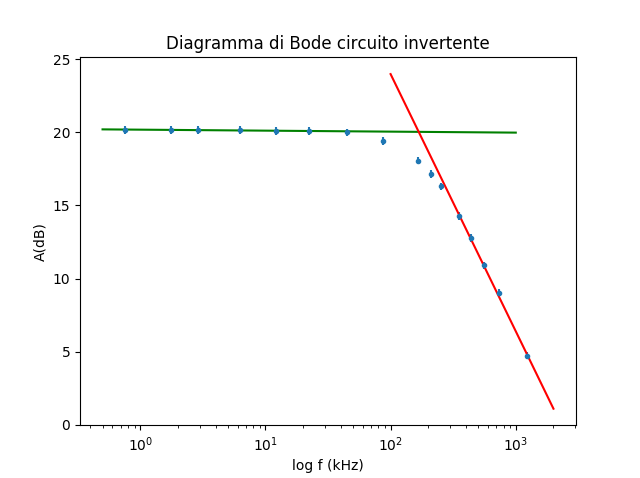
\includegraphics[width=0.7\textwidth]{bodeInvertente}
			\caption{\small Plot di Bode in ampiezza per l'~amplificatore invertente.}
			\label{fig:bodeinv}
		\end{center}
	\end{figure}
	%
	\subsection{Misura dello \emph{slew-rate}}
	Si misura direttamente lo \emph{slew-rate} dell'op-amp inviando in ingresso un'~onda quadra 
	di frequenza intorno ai $\sim 0.9$~kHz e di ampiezza $2.08$~V. Si ottiene:
	\[
	SR_\mathrm{misurato} = (12.5 \pm 0.5 )\,\mathrm{V/\mu s} \quad \mathrm{valore \; tipico}\, (13 )\,\mathrm{V/\mu s}\
	\]

Abbiamo misurato la  pendenza massima del segnale $V_{out}$, che si trova proprio  in corrispondenza dell' inizio dell'onda quadra, subito dopo la pendenza diminuisce di circa 0.5 $ \mathrm{V/\mu s}$

\begin{figure}[h]
		\begin{center}
			
			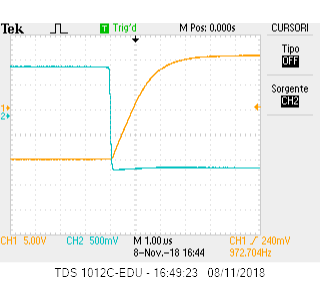
\includegraphics[width=0.7\textwidth]{slewrate}
			\caption{\small Segnale onda quadra (azzurro) e $V_{in}$ (arancio)}
			\label{fig:Slew  Rate}
		\end{center}
	\end{figure}

\clearpage
	\section{Circuito integratore}
	Si monta il circuito integratore con i seguenti valori  dei componenti indicati: 
	\[
	R_1 = (0.997 \pm 0.008 \;) \,\mathrm{k}\Omega, \:\:\;\:\exn 
	R_2 = (9.92 \pm 0.08 \;) \,\mathrm{k}\Omega, \:\:\;\:\exn 
	C = (50.4 \pm 2.3 \;\;)\,\mathrm{nF}
	\]
	
	\subsection{Risposta in frequenza}
	

	\begin{figure}[h]
	\begin{center}
		
		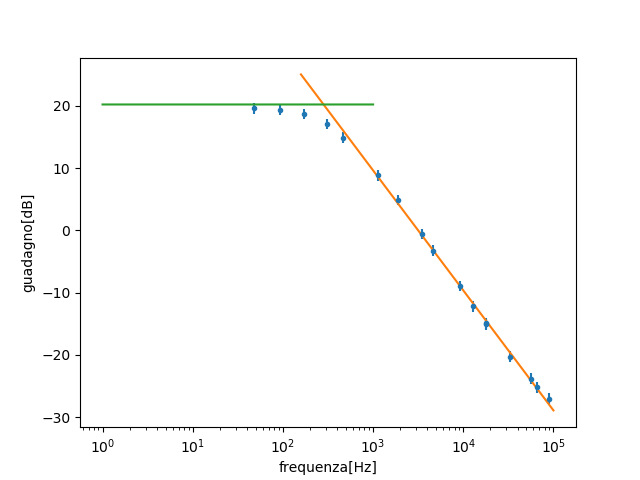
\includegraphics[scale=0.5]{bodefrequenza.png}		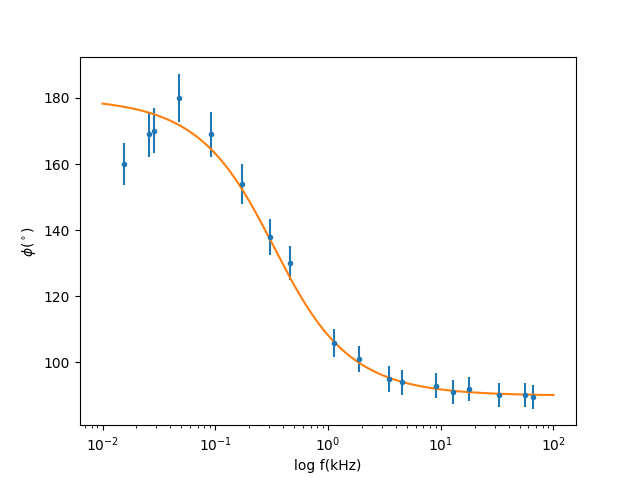
\includegraphics[scale=0.5]{fase.png}
		
		
	\end{center}
	\caption{\small Plot di Bode in ampiezza (a sinistra) e fase (a destra) per il circuito integratore.}
	\label{fig:bodeinte}
\end{figure}

	Si invia un'~onda sinusoidale e si misura la risposta in frequenza dell'~amplificazione e della fase.
	I dati sono riportati in tabella \ref{tab:bodeinte} e \ref{tab:bodefase}.

         Si vedano le figure \ref{fig:bodeinte} e 7, per i plot di Bode dell'integratore relativi ad ampiezza e fase.

	%





	\begin{table}[h]
		\caption{Guadagno  dell'~integratore invertente in funzione della frequenza.}
		\label{tab:bodeinte}
		\begin{center}
			\begin{tabular}{|c|c|c|c|}
				\hline
				$f_{in}$ (kHz) &$V_{in}$(V) & $V_{out}$ (V) & $A$ (dB)  \\
				\hline









				$\exn(1.56 \pm0.03)\cdot 10^{-2} \exn $ &$\exn0.580 \pm 0.017\exn $ & $\exn5.12 \pm 0.15\exn $ & $\exn 18.9\pm0.26 \exn $ \\
				\hline
				$\exn ( 2.57\pm0.05)\cdot 10^{-2} \exn $ &$\exn0.580 \pm 0.017 \exn $ & $\exn5.44 \pm0.15 \exn $ & $\exn 19.4\pm 0.26\exn $ \\

					
				\hline
				$\exn(2.87 \pm0.06)\cdot 10^{-2} \exn $ &$\exn 0.580\pm0.017\exn $ & $\exn 5.52 \pm0.15 \exn $ & $\exn 19.6\pm0.26 \exn $ \\

				\hline
				$\exn (4.79\pm0.01)\cdot 10^{-2} \exn $ &$\exn1.53 \pm 0.05\exn $ & $\exn 14.6 \pm0.5 \exn $ & $\exn 19.6\pm 0.26\exn $  \\
				
				\hline
				$\exn(9.20\pm 0.2)\cdot 10^{-2}\exn $ &$\exn1.54\pm 0.05\exn $ & $\exn 14.3\pm0.4\exn $ & $\exn 19.4\pm 0.26\exn $ \\
				\hline

				$\exn0.172 \pm0.003 \exn $ &$\exn1.54 \pm0.05 \exn $ & $\exn 13.2 \pm 0.4\exn $ & $\exn 18.7\pm0.26 \exn $  \\
				\hline
				$\exn0.306 \pm0.006 \exn $ &$\exn 1.53\pm0.05 \exn $ & $\exn 10.9\pm 0.3\exn $ & $\exn 17.0\pm0.26 \exn $  \\
				\hline
				
				
				
				$\exn 0.460\pm0.05 \exn $ &$\exn 0.704 \pm0.021 \exn $ & $\exn3.92 \pm 0.12\exn $ & $\exn14.9 \pm0.26 \exn $  \\
				\hline
				$\exn 1.14\pm 0.02\exn $ &$\exn 0.700\pm0.021 \exn $ & $\exn 1.94\pm0.08 \exn $ & $\exn8.85 \pm0.26 \exn $ \\
				\hline
				$\exn 1.88\pm0.04 \exn $ &$\exn 0.696 \pm0.020 \exn $ & $\exn1.22 \pm 0.04 \exn $ & $\exn4.87 \pm0.26 \exn $  \\
				\hline
				$\exn 3.46\pm 0.07 \exn $ &$\exn 0.704 \pm0.020 \exn $ & $\exn 0.656\pm0.018 \exn $ & $\exn-0.613 \pm 0.26\exn $\\
				\hline
				$\exn4.57 \pm0.09 \exn $ &$\exn 1.56\pm 0.05\exn $ & $\exn1.07 \pm 0.3\exn $ & $\exn-3.27 \pm 0.26\exn $ \\
				\hline

				$\exn 9.14\pm 0.20\exn $ &$\exn 0.712\pm0.021 \exn $ & $\exn0.255 \pm 0.007\exn $ & $\exn -8.92\pm 0.26\exn $  \\
				\hline

				$\exn 12.9\pm 0.2 \exn $ &$\exn 1.55\pm0.05 \exn $ & $\exn0.380 \pm 0.012\exn $ & $\exn -12.2\pm 0.26\exn $  \\
				\hline
				$\exn 17.7\pm 0.3\exn $ &$\exn 3.92\pm0.12 \exn $ & $\exn 0.688\pm 0.020\exn $ & $\exn -15.1\pm 0.26\exn $ \\

				\hline
				$\exn 33\pm 0.6\exn $ &$\exn 3.92 \pm 0.12\exn $ & $\exn0.380 \pm 0.012\exn $ & $\exn -20.2\pm0.26 \exn $ \\
				\hline
				$\exn 56\pm 1 \exn $ &$\exn 0.696\pm0.020 \exn $ & $\exn (4.48\pm0.12)\cdot 10^{-2} \exn $ & $\exn-23.8\pm 0.26\exn $ \\
				
				
				\hline
				$\exn 66.1\pm 1.2\exn $ &$\exn 3.86\pm 0.12\exn $ & $\exn0.212 \pm0.006 \exn $ & $\exn -25.2\pm0.26 \exn $  \\
			
				
				\hline
				
				
				
				
			\end{tabular}
		\end{center}
	\end{table} 





\begin{figure}
		\caption{\small andamento dei punti sperimentali e modello per la fase in funzione della frequenza.}
	
	\label{esempio}
	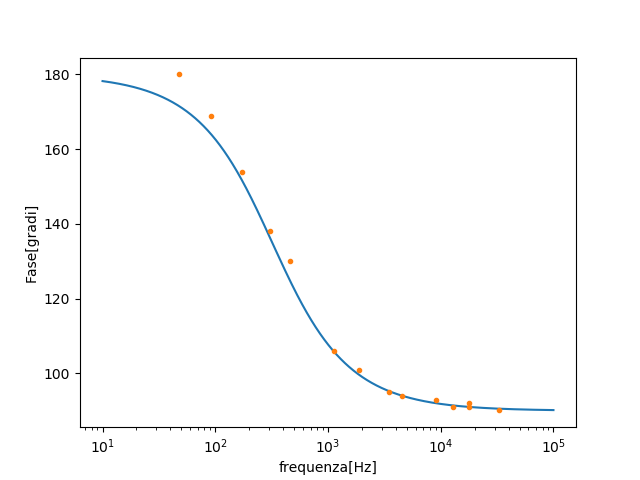
\includegraphics[scale=0.5]{esempio.png}
\end{figure}
	


	%
	
	Si ricava una stima delle caratteristiche principali dell'andamento (guadagno a bassa frequenza, frequenza di taglio, e pendenza ad alta frequenza)
	e si confrontano con quanto atteso. Non si effettua la stima degli errori, trattandosi di misure qualitative.
	La frequenza di taglio viene stimata come al solito con l'intesezione delle due rette; una delle due è stata determinata con un fit lineare, mentre per disegnare la retta del guadagno massimo si è usato il valore misurato in precedenza di $A\approx10.26$. Il valore della frequenza di taglio così ottenuto è $f_t\approx0.32 kHz$, in accordo con la frequenza di taglio che ci si aspetterebbe $f_t=\frac{1}{2\pi R_2C}=0.32\pm0.01 kHz$. Si può trascurare del tutto la frequenza di taglio del'opamp,che è tre decadi più avanti.
	L'andamento della fase pure è quello che ci si aspetta, dato che per alte frequenze lo sfasamento deve essere di 90 $^{\circ}$ (domina l'impedenza del condensatore che sfasa di j), mentre per basse frequenze è quella solita di 180$^{\circ}$ di un amplificatore invertente. L'andamento teorico può essere descritto da una formula del tipo:\[\Delta\phi=180^{\circ}-arctan(f/f_t)\]. usando il valore di $f_t$ stimato prima si può notare un discreto accordo con i dati, come riportato in figura \ref{esempio}
	

	
	\begin{table}[h]
		\caption{ fase dell'~integratore invertente in funzione della frequenza.}
		\label{tab:bodefase}
\centering
		

			\begin{tabular}{|c|c|c|}
				\hline
				$f_{in}$ (kHz)  & $\Delta t (\mu s)$ & $\phi \,(\,\,^\circ)$ \\
				\hline


				$\exn(1.56 \pm0.03)\cdot 10^{-2} \exn $& $\exn (28.4\pm 1.1)\cdot 10^3  \exn $ & $\exn160 \pm6\exn $ \\
				\hline
				$\exn( 2.57\pm0.05)\cdot 10^{-2} \exn $ &$\exn (18.2\pm 0.7)\cdot 10^3  \exn $ & $\exn169 \pm 7 \exn $ \\

					
				\hline
				$\exn(2.87 \pm0.06)\cdot 10^{-2} \exn $  & $\exn(16.4 \pm   0.7)\cdot 10^3 \exn $ & $\exn 170\pm 7\exn $ \\

				\hline
				$\exn (4.79\pm0.01)\cdot 10^{-2} \exn $ & $\exn(10.4 \pm 0.4)\cdot 10^3 \exn $ & $\exn 180\pm 7 \exn $ \\
				
				\hline
				$\exn (9.20\pm 0.2)\cdot 10^{-2}\exn $  & $\exn (5.1\pm 0.2)\cdot 10^3 \exn $ & $\exn169\pm7\exn $ \\
				\hline

				$\exn0.172 \pm0.003 \exn $  & $\exn (2.49\pm   0.1)\cdot 10^3   \exn $ & $\exn 154\pm6 \exn $ \\
				\hline
				$\exn0.306 \pm0.006 \exn $  & $\exn (1.25 \pm 0.05)\cdot 10^3  \exn $ & $\exn138 \pm 6\exn $ \\
				\hline
				
				
				
				$\exn 0.460\pm0.05 \exn $& $\exn785 \pm 30 \exn $ & $\exn130 \pm5  \exn $ \\
				\hline
				$\exn 1.14\pm 0.02\exn $  & $\exn258 \pm  10  \exn $ & $\exn106 \pm 4\exn $ \\
				\hline
				$\exn 1.88\pm0.04 \exn $  & $\exn 149 \pm  6 \exn $ & $\exn101 \pm 4 \exn $ \\
				\hline
				$\exn 3.46\pm 0.07 \exn $  & $\exn 76.3 \pm3
   \exn $ & $\exn95 \pm 4\exn $ \\
				\hline
				$\exn4.57 \pm0.09 \exn $  & $\exn 57.1 \pm  2.3    \exn $ & $\exn94 \pm4\exn $ \\
				\hline

				$\exn 9.14\pm 0.20\exn $ & $\exn28.2 \pm 1.1   \exn $ & $\exn 93 \pm 4 \exn $ \\
				\hline

				$\exn 12.9\pm 0.2 \exn $  & $\exn 19.6 \pm 0.8 \exn $ & $\exn 91 \pm  4\exn $ \\
				\hline
				$\exn 17.7\pm 0.3\exn $ & $\exn14.4\pm 0.6 \exn $ & $\exn 92\pm4\exn $ \\

				\hline
				$\exn 33\pm 0.6\exn $& $\exn7.58 \pm  0.3
   \exn $ & $\exn90 \pm 4 \exn $ \\
				\hline
				$\exn 56\pm 1 \exn $  & $\exn 4.47\pm0.18   \exn $ & $\exn 90\pm 4\exn $ \\
				
				
				\hline
				$\exn 66.1\pm 1.2\exn $ & $\exn3.76 \pm  0.15 \exn $ & $\exn90 \pm 4\exn $ \\
			
				
				\hline
				
				
				
				
			\end{tabular}
\end{table}


	%
\begin{figure}[h]
		\begin{center}
			
			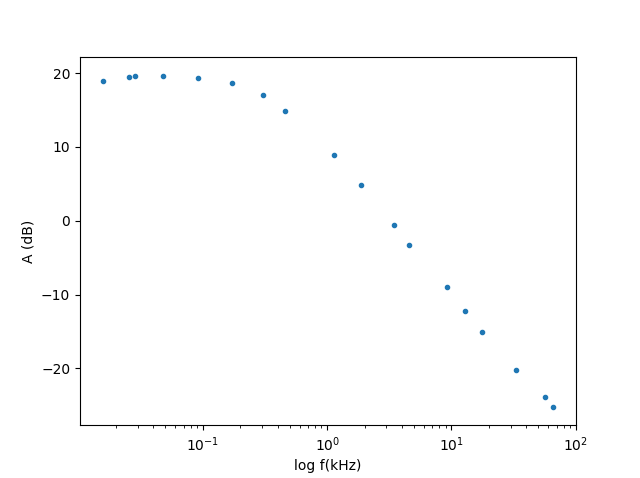
\includegraphics[width=0.7\textwidth]{bodeint}
			
	\end{center}
		\caption{\small Plot di Bode dell' ampiezza  per il circuito integratore.}
		\label{fig:bodeinte}
\end{figure}

         \begin{figure}[h]
                                       
		\begin{center}
			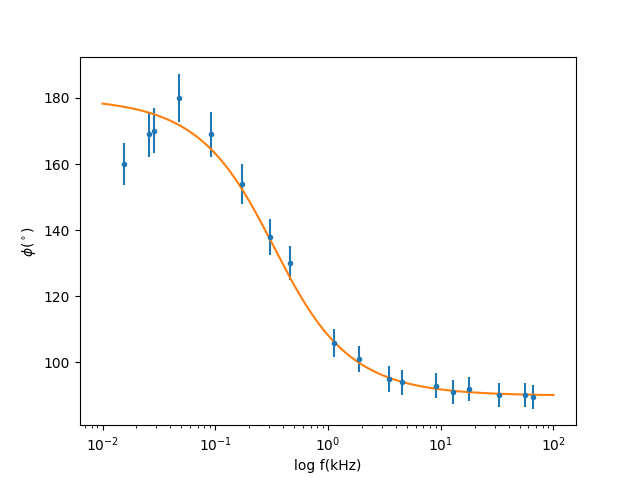
\includegraphics[width=0.7\textwidth]{fase}
			 \label{fig:fase}
		\end{center}
		\caption{\small Plot di Bode della fase per il circuito integratore}
		
	\end{figure}
	%
	 
	Per la stima del guadagno massimo, si è presa la media dei guadagni delle prime quattro frequenze.


	Guardando per quale $f$ il guadagno fosse  $A_M - 3 $dB si è ottenuta una stima della frequenza di taglio.

	Per la pendenza abbiamo preso una media delle pendenze delle rette passanti per coppie di punti ad alte frequenze.

	Il valore atteso per $A_M $ è $ 20 \log_{10}(R_2/R_1)$; la frequenza di taglio attesa è $f_H = 1/(2\pi R_2 C)$.


	
	\begin{align*}
	A_M &= (19.4 )\,\mathrm{dB} & \mathrm{atteso} &:\,(20  )\, \mathrm{dB}  \\
	f_H &= (330 )\,\mathrm{Hz} & \mathrm{atteso} &:\,(318  )\, \mathrm{Hz} \\
	{\mathrm{d}A_V}/{\mathrm{d}f} &= (-20.1 )\,\mathrm{dB/decade} & \mathrm{atteso} &:\,(-20  )\, \mathrm{dB/decade}  \\
	\end{align*}
	
	\clearpage
	%
	\subsection*{Risposta ad un'~onda quadra}
	Si invia all'~ingresso un'~onda quadra di frequenza $\sim 10.0\pm0.7 \,kHz$ e ampiezza $\sim 1.40\pm 0.05\,V$.
	Si riporta in Fig. \ref{fig:oscinte} le forme d'~onda acquisite all'~oscillografo per l'~ingresso
	e l'~uscita. 
	Come atteso per un integratore, l'uscita è costituita da onde triangolari.
	%
	\begin{figure}[htb]
		\begin{center}

			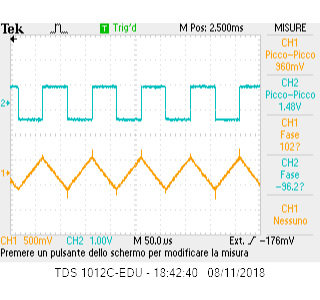
\includegraphics[scale=0.8]{zanna.png}
		\end{center}
		\caption{\small Ingresso (in alto) ed uscita (in basso) del circuito integratore per un'~onda quadra.}
		\label{fig:oscinte}
	\end{figure}
	%
	
	Si misura l'~ampiezza dell'~onda  in uscita e si confronta il valore atteso.
	
	\begin{align*}
	V_{out pp} &= (0.66\pm 0.03 )\,\mathrm{V} & \mathrm{atteso} &:\,(0.67\pm 0.05 )\, \mathrm{V}  \\
	\end{align*}
 	Ci si aspetta infatti, per un'onda quadra in ingresso, con un integratore perfetto (trascurando cioè l'effetto di $R_2$),una relazione del tipo: \[V_{out}=\frac{V_{in}}{4fR_{1}C}\]
	%
	\clearpage
	\subsection{Discussione}
	

	Si è poi provato a variare la frequenza fino a valori intorno, e sotto, la frequenza di taglio. A questo punto il segnale in uscita risultava distorto rispetto all'onda triangolare. Per frequenze al di sotto la frequenza di taglio, il segnale in uscita è costituito sostanzialmente dalle scariche del condensatore, come riportato ad esempio in Figura \ref{fig:scariche}.
	Per frequenze ancora al di sotto, come in Figura \ref{fig:lowf} si osserva un segnale discontinuo in uscita, il che è sorprendente dato che il segnale che si osserva è sostanzialmente proporzionale alla carica sul condensatore, e quindi lo si aspetta continuo.  In realtà quello che succede è che, dato che il segnale è molto amplificato, al cambio di polarità dell'onda quadra, il condensatore si scarica su $R_1$, anzichè su $R_2$, e, dato che $R_1$ è 10 volte più piccola, lo fa con una velocità 10 volte più grande rispetto al solito, il che sembra un processo istantaneo, per la scala dei tempi a cui è impostato l'oscilloscopio, . Finita la scarica su $R_1$ si osserva quella solita su $R_2$. 
	\begin{figure}[h]

			\centering
			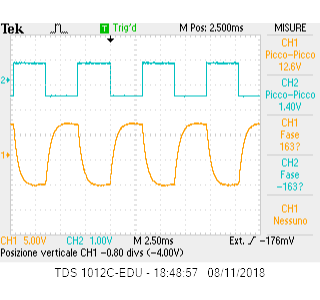
\includegraphics[scale=1]{scariche.png}

			\caption{segnale a "pinna di squalo"}
						\label{fig:scariche}

	\end{figure}
	\begin{figure}[h]
\centering
		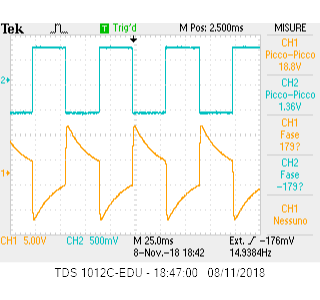
\includegraphics[scale=1]{lowf.png}
					\caption{segnale a bassa frequenza}
		\label{fig:lowf}
		
	\end{figure}
	%%%%%%%%%%%%%%%%%%%%%%%%
	
	
	
	

	\rem{Inserire commenti su quanto osservato ed eventuali deviazioni. 
		In particolare: attenuazione ad alte frequenze, dipendenza della fase dalla frequenza, funzione di $R_2$. }

 Per i valori teorici attesi abbiamo usato $V_{out}= -\frac{Z_2}{Z_1} V_{in}$ e quindi implicitamente abbiamo considerato valida anche ad alte  frequenze l'approssimazione $A_d \gg |\frac{Z_2}{Z_1}|$. Effettivamente per grandi $f$  $A_d\propto 1/f$ (punto 2.a) ma anche l'impedenza del condensatore decresce come $1/f$, di conseguenza l'approssimazione resta valida.
	In figura 7  la linea arancione rappresenta il comportamento teorico della fase; che è descritto dalla funzione \[ \phi = 360/(2\pi)[\pi - \arctan(10^{(\log f -\log f_t)})\] 

Per basse frequenze i dati hanno una evidente deviazione da quanto atteso; questo è sicuramente dovuto a un nostro errore di presa dati.

	%%%%%%%%%%%%%%%%%%%%%%%%
	\begin{tabular}{cc}

\end{tabular}


\end{document}          
